\documentclass[11pt,compress,t,notes=noshow, aspectratio=169, xcolor=table]{beamer}
\newcommand{\btVFill}{\vskip0pt plus 1filll}
\newcommand\hmmax{0}
\newcommand\bmmax{0}
\usepackage{../../style/lmu-lecture}
\usepackage{siunitx}
% Defines macros and environments
% This file is included in slides and exercises

% Rarely used fontstyle for R packages, used only in 
% - forests/slides-forests-benchmark.tex
% - exercises/single-exercises/methods_l_1.Rnw
% - slides/cart/attic/slides_extra_trees.Rnw
\newcommand{\pkg}[1]{{\fontseries{b}\selectfont #1}}

% Spacing helpers, used often (mostly in exercises for \dlz)
\newcommand{\lz}{\vspace{0.5cm}} % vertical space (used often in slides)
\newcommand{\dlz}{\vspace{1cm}}  % double vertical space (used often in exercises, never in slides)
\newcommand{\oneliner}[1] % Oneliner for important statements, used e.g. in iml, algods
{\begin{block}{}\begin{center}\begin{Large}#1\end{Large}\end{center}\end{block}}

% Don't know if this is used or needed, remove?
% textcolor that works in mathmode
% https://tex.stackexchange.com/a/261480
% Used e.g. in forests/slides-forests-bagging.tex
% [...] \textcolor{blue}{\tfrac{1}{M}\sum^M_{m} [...]
% \makeatletter
% \renewcommand*{\@textcolor}[3]{%
%   \protect\leavevmode
%   \begingroup
%     \color#1{#2}#3%
%   \endgroup
% }
% \makeatother


\title{Interpretable Machine Learning}
% \author{LMU}
%\institute{\href{https://compstat-lmu.github.io/lecture_iml/}{compstat-lmu.github.io/lecture\_iml}}
\date{}

\begin{document}

% TODO
\newcommand{\titlefigure}{figure_man/exSHAP.png}
\newcommand{\learninggoals}{
\item Get an intuition of additive feature attributions
\item Understand the concept of Kernel SHAP
\item Ability to interpret SHAP plots
\item Global SHAP methods
}

\lecturechapter{SHAP (SHapley Additive exPlanation) Values}
\lecture{Interpretable Machine Learning}

\begin{frame}{Shapley Values in ML - A short Recap}
  
  \textbf{Question:} How much does a feat. $j$ contribute to the prediction of a single obs. \\
  \textbf{Idea:} Use Shapley values from cooperative game theory \\
  \pause
  \textbf{Procedure:} 
  \begin{itemize}
    \item Compare ``reduced prediction function'' of feature coalition $S$ with $\Scupj$ 
    \item Iterate over possible coalitions to calculate marginal contribution of feature $j$ to sample $\xv$
\end{itemize}

$$\phi_j 
%= \frac{1}{|P|!} \sum_{\tau \in \Pi} (v(\Stauj) - v(\Stau)) 
= \frac{1}{p!} \sum_{\tau \in \Pi}  \underbrace{\fh_{\Stauj}(\xv_{\Stauj}) - \fh_{\Stau}(\xv_{\Stau})}_{\text{marginal contribution of feature $j$}} $$

\pause
\textbf{Remember:}

\begin{itemize}
    \item $\fh$ is the prediction function, $p$ denotes the number of features
    \item Non-existent feat. in a coalition are replaced by values of random feat. values 
    \item Recall $\Stau$ defines the coalition as the set of players before player $j$ in order $\tau = (\tau^{(1)}, \dots, \tau^{(p)})$% states from the feature
    
  \centerline{
  \begin{tabular}{|c|c|c|c|c|c|c|}
    %\multicolumn{3}{c}{\enspace\raisebox{-3.3ex}[0pt][2.6ex]{$ \overbrace{\vphantom{-}\hspace{9em}}^{|S|! \text{ permutations}}$}} &
    %\multicolumn{1}{c}{} &
    %\multicolumn{3}{c}{\enspace\raisebox{-3.3ex}[0pt][2.6ex]{$ \overbrace{\vphantom{-}\hspace{9em}}^{(|P| - |S| - 1)! \text{ permutations}}$}}\\
    \hline
    $\tau^{(1)}$ & \ldots & $\tau^{(|S|)}$ & $\tau^{(|S| + 1)}$ & $\tau^{(|S| + 2)}$ & \ldots & $\tau^{(p)}$ \\
    \hline
    \multicolumn{3}{c}{\enspace\raisebox{1.3ex}[0pt][2.6ex]{$ \underbrace{\vphantom{-}\hspace{9em}}^{}$}} &
    \multicolumn{1}{c}{\enspace\raisebox{1.3ex}[0pt][2.6ex]{$ \underbrace{\vphantom{-}\hspace{4em}}^{}$}} &
    \multicolumn{3}{c}{\enspace\raisebox{1.3ex}[0pt][2.6ex]{$ \underbrace{\vphantom{-}\hspace{9em}}^{}$}}\\
    \multicolumn{3}{c}{$S_j^\tau:$ Players before player $j$} & \multicolumn{1}{c}{player $j$} & \multicolumn{3}{c}{Players after player $j$} \\
  \end{tabular}}
\end{itemize}

\end{frame}


\begin{frame}{Shapley Values in ML - A short Recap}
  
  \textbf{Example:} 
  \begin{itemize}
      \item Train a random forest on bike sharing data only using features humidity (hum), temperature (temp) and windspeed (ws)
      \item Calculate Shapley value for an observation $\xv$ with $\fh(\xv) = \color{orange}{2573}$
      \item Mean prediction is $\E(\fh) = \color{blue}{4515}$
  \end{itemize}
  \pause
  \textbf{Exact Shapley calculation for humidity:} 
  \begin{table}[T]
      \centering
      \begin{tabular}{c|c|c|c|c}
   $S$    &  $\Scupj$  & $\fh_S$ &  $\fh_{\Scupj}$  & weight\\\hline
     $\varnothing$&    hum  & \color{blue}{4515} & 4635 & $2/6$\\
       temp &  temp, hum & 3087 & 3060& $1/6$\\
       ws &  ws, hum & 4359  & 4450 & $1/6$\\
       temp, ws & temp, ws, hum & 2623 & \color{orange}{2573} & $2/6$
         
      \end{tabular}
      \label{tab:my_label}
  \end{table}

$$
\phi_{hum} = \frac{2}{6} (4635-4515) + \frac{1}{6} (3060-3087) + \frac{1}{6} (4450-4359) + \frac{2}{6} (2573-2623) = 34
$$

\end{frame}


\begin{frame}{From Shapley to SHAP}
\textbf{Example continued}: Same calculation can be done for temperature and windspeed:
\begin{itemize}
    \item $\phi_{temp} = \ldots = -1654$
    \item $\phi_{ws} = \ldots = -322$
\end{itemize}

\textbf{Remember}: Shapley values explain difference between actual and average pred.:
\begin{eqnarray*}
\color{orange}{2573} \color{black}- \color{blue}{4515} \color{black} &= 34 - 1654 - 322 &= - 1942\\
\fh(\xv) - \E(\fh) &= \phi_{hum} + \phi_{temp} + \phi_{ws}&\\
\end{eqnarray*}
\begin{columns}[T]
\begin{column}{0.5\textwidth}
$\leadsto$ can be rewritten to
$$
\fh(\xv) = \underbrace{\E(\fh)}_{\phi_0} + \phi_{hum} + \phi_{temp} + \phi_{ws}
$$
%N.B.: This reminds us of a LM with weights $\phi_j$ multiplied by a binary feature value indicating weather a feature is included in a considered coalition.
\end{column}
\begin{column}{0.5\textwidth}
\vspace{-1cm}
\begin{figure}
    \centering
    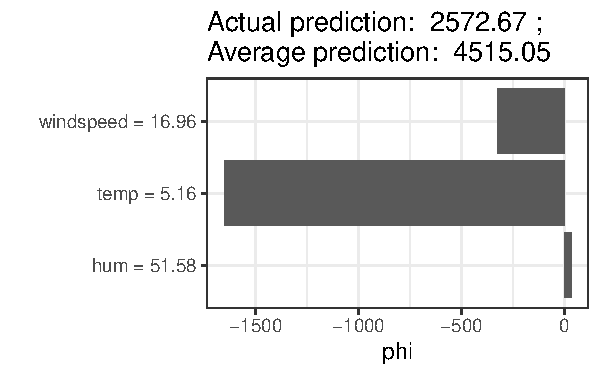
\includegraphics[width=0.9\columnwidth]{figure/shapley2shap.pdf}
\end{figure}
\end{column}
\end{columns}
\end{frame}



\begin{frame}{SHAP Definition \citebutton{Lundberg et al. 2017}{https://doi.org/10.48550/arXiv.1705.07874}}
\textbf{Aim}: 
Find an additive combination that explains the prediction of an observation $\xv$ by computing the contribution of each feature to the prediction using a (more efficient) estimation procedure. \\\medskip
\only<1-4>{\textbf{Definition}
\begin{itemize}
    \item Simplified (binary) coalition feat. space $\mathbf{Z}^\prime \in \{0,1\}^{K \times p}$ with $K$ rows and $p$ cols.
    \item Rows are referred to as $\mathbf{z}^{\prime (k)} = \{z^{\prime (k)}_1, \ldots, z^{\prime (k)}_p\}$ with $k \in \{1,\ldots, K\}$ (indexes $k$-th coalition)
    \item Cols are referred to as $\mathbf{z}_j$ with $j \in \{1, \ldots, p\}$ being the index of the original feat.
\end{itemize}
}
\only<1>{
\textbf{Example}: 
\vspace{-0.2cm}
\begin{table}[]
    \centering
    \footnotesize
     \begin{tabular}{l |c|ccc}
  Coalition  & $\mathbf{z}^{\prime (k)}$ &  hum & temp & ws \\
  \hline 
  $\varnothing$ & $\mathbf{z}^{\prime (1)}$ & 0 & 0 & 0  \\
  hum & $\mathbf{z}^{\prime (2)}$ & 1 & 0 & 0  \\
  temp &  $\mathbf{z}^{\prime (3)}$ & 0 & 1 & 0  \\
  ws &   $\mathbf{z}^{\prime (4)}$ & 0 & 0 & 1  \\
  hum, temp & $\mathbf{z}^{\prime (5)}$ & 1 & 1 & 0  \\
  temp, ws & $\mathbf{z}^{\prime (6)}$ & 0 & 1 & 1  \\
  hum, ws &   $\mathbf{z}^{\prime (7)}$ & 1 & 0 & 1  \\
  hum, temp, ws & $\mathbf{z}^{\prime (8)}$ & 1 & 1 & 1  \\
  \end{tabular}
\end{table}
}
\only<2->{
%\vspace{0.5cm}
\begin{exampleblock}{}
\[
g\left(\tikzmark{zp} \mathbf{z}^{\prime (k)}\right)=
\tikzmark{ph0}\phi_{0}+\sum_{j=1}^{p}
\tikzmark{phj} \phi_{j} z_{j}^{\prime (k)}
\]
\begin{tikzpicture}[
  remember picture,
  overlay,
  expl/.style={draw=blue,fill=white,rounded corners,text width=3cm},
  arrow/.style={blue,ultra thick,->,>=latex}
]
\node<2-4>[expl] 
  (zex) 
  at (2,1.5cm)
  {$\mathbf{z}^{\prime (k)}$: \textbf{Coalition} \\ simplified features};
\node<3-4>[expl] 
  (ph0ex) 
  at (4,-.5cm)
  {$\phi_0$: \textbf{Null Output} \\ Average Model Baseline ($\E(\fh))$};
\node<4>[expl] 
  (phjex) 
  at (10,0cm)
  {$\phi_j$: \textbf{Attribution} \\ How much does feature $j$ change the output for coaltion $k$};

\draw<2-4>[arrow]
  (zex.east) to[out=0,in=120] ([xshift= 1ex, yshift=2.3ex]{pic cs:zp});  
\draw<3-4>[arrow]
  (ph0ex.east) to[out=0,in=270] ([xshift= 1ex, yshift=-0.8ex]{pic cs:ph0});  
\draw<4>[arrow]
  (phjex.west) to[out=180,in=270] ([xshift= 1ex, yshift=-1ex]{pic cs:phj});
 \node<5>[expl] 
  (zex)  
  at (2,1cm)
  {$g(\mathbf{z}^{\prime (k)})$: \textbf{Marginal Contribution} \\ Contribution of coalition $\mathbf{z}^{\prime (k)}$ to the prediction};
  \draw<5>[arrow]
  (zex.east) to[out=0,in=140] ([xshift= 1ex, yshift=2.3ex]{pic cs:zp});  
\node<5>[expl] 
  (phjsh) 
  at (10,1.5cm)
  {$\phi_j$: \textbf{Shapley Values}};
\draw<5>[arrow]
  (phjsh.west) to[out=180,in=50] ([xshift= 1ex, yshift=2ex]{pic cs:phj}); 
\draw<5> [
    thick,
    decoration={
        brace,
        mirror,
        raise=0.5cm
    },
    decorate
] (5.7,0.7) -- (8.2,0.7)
node[pos=0.5,below=15pt,black]{\textbf{Additive Feature Attribution}};
\end{tikzpicture}
\end{exampleblock}
\begin{onlyenv}<5>
\vspace{1cm}
\textbf{Problem}\\
How do we estimate the Shapley values $\phi_j$?
\end{onlyenv}}

\end{frame}



%\begin{frame}{Example}

%Given the following example from the bike sharing data set

%\begin{table}[h]
%\centering
%\begin{tabular}{l rrrrr || r}
%  \hline
%  && temperature & humidity & windspeed & year & prediction\\ 
%  \hline
% example $x_{ex}$ && 24.27 & 58.5 & 13.96 & 2011 & 6825 \\ 
% \hline
%\end{tabular}
%\end{table}

%we are searching for Shapley values such that
%\begin{equation}
%\begin{array}{lllllcr}
%\phi_0 &+ \phi_{temp} &+ \phi_{hum} &+ \phi_{windspeed} &+ \phi_{yr} & = &\hat{y} \\
%4469 &+ 1809 &+ 450 &+ 241 &- 144 & = & 6825
%\end{array}
%\end{equation}

%\begin{figure}
 %   \centering
 %   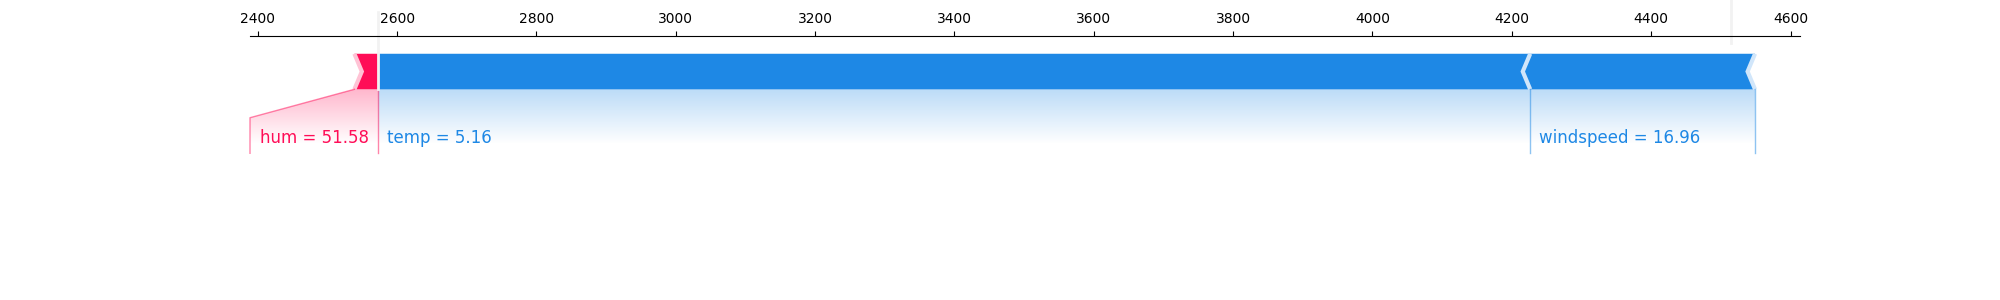
\includegraphics[width=\columnwidth]{figure_man/exSHAP.png}
%\end{figure}
%\end{frame}

% \begin{frame}{Kernel SHAP - In 5 Steps}

% \textbf{Definition:} A kernel-based, model-agnostic method to compute Shapley values via local surrogate models (e.g. linear model)\\
% \vspace{1cm}
% \begin{enumerate}
%     \item Sample coalitions 
%     %\begin{onlyenv}<1>
%    % $$z_{k}^{\prime} \in\{0,1\}^{M}, \quad k \in\{1, \ldots, K\}$$
%     %\end{onlyenv}
    
%     \item Transfer coalitions into feature space \& get predictions by applying ML model
    
%  %   \begin{onlyenv}<2>
%   %  $$\hat{f}: \hat{f}\left(h_{x}\left(z_{k}^{\prime}\right)\right)$$
%    % \end{onlyenv}
    
%     \item Compute weights through kernel
%  %   \begin{onlyenv}<3>
%  %   $$\pi_{x}\left(z^{\prime}\right)=\frac{(M-1)}{\left(\begin{array}{c} M \\\left|z^{\prime}\right|\end{array}\right)\left|z^{\prime}\right|\left(M-\left|z^{\prime}\right|\right)}$$
%  %   \end{onlyenv}
    
%     \item Fit a weighted linear model 
%   %  \begin{onlyenv}<4>
%   %  $$L\left(\hat{f}, g, \pi_{x}\right)=\sum_{z^{\prime} \in Z}\left[\hat{f}\left(h_{x}\left(z^{\prime}\right)\right)-g\left(z^{\prime}\right)\right]^{2} \pi_{x}\left(z^{\prime}\right)$$
%   %  \end{onlyenv}

%     \item Return Shapley values
% %    \begin{onlyenv}<5>
% %    $$(\phi_1, \ldots, \phi_M)$$
% %    \end{onlyenv}
    
    
% \end{enumerate}

% \end{frame}

% \begin{frame}{Kernel SHAP - In 5 Steps}


% \textbf{Step 1: Sample coalitions}
% \begin{itemize}
%     \item Sample K coalitions from the simplified feature space
%     $$\mathbf{z}^{\prime (k)} \in\{0,1\}^{p}, \quad k \in\{1, \ldots, K\}$$
%     \item For our simple example, we have in total $2^p = 2^3 = 8$ coalitions (without sampling)
% \end{itemize}

% \begin{table}[]
%     \centering
%      \begin{tabular}{l |c|ccc}
%   Coalition  & $\mathbf{z}^{\prime (k)}$ &  hum & temp & ws \\
%   \hline 
%   $\varnothing$ & $\mathbf{z}^{\prime (1)}$ & 0 & 0 & 0  \\
%   hum & $\mathbf{z}^{\prime (2)}$ & 1 & 0 & 0  \\
%   temp &  $\mathbf{z}^{\prime (3)}$ & 0 & 1 & 0  \\
%   ws &   $\mathbf{z}^{\prime (4)}$ & 0 & 0 & 1  \\
%   hum, temp & $\mathbf{z}^{\prime (5)}$ & 1 & 1 & 0  \\
%   temp, ws & $\mathbf{z}^{\prime (6)}$ & 0 & 1 & 1  \\
%   hum, ws &   $\mathbf{z}^{\prime (7)}$ & 1 & 0 & 1  \\
%   hum, temp, ws & $\mathbf{z}^{\prime (8)}$ & 1 & 1 & 1  \\
  
 
%   \end{tabular}
% \end{table}

% \end{frame}

% \begin{frame}{Kernel SHAP - In 5 Steps}


% \textbf{Step 2: Transfer Coalitions into feature space \& get predictions by applying ML model}
% \begin{itemize}
%    % \item $$\hat{f}: \hat{f}\left(h_{x}\left(z_{k}^{\prime}\right)\right)$$
%    \item $\mathbf{z}^{\prime (k)}$ is 1 if features are are part of the $k$-th coalition, 0 if they are absent
%    \item To calculate predictions for these coalitions, we need to define a function which maps the binary feature space back to the original feature space
% \end{itemize}


% \begin{tikzpicture}
% \centering

% \fontsize{8}{12}

% \node (tab1) {%
%        \begin{tabular}{l |cccc}
%   $\xv^{coalition}$ &  hum & temp & ws \\
%   \hline 
%   $\xv^{\{\varnothing\}}$ & $\varnothing$ & $\varnothing$ &$\varnothing$  \\
%    $\xv^{\{hum\}}$ & 51.6 & $\varnothing$ & $\varnothing$  \\
%     $\xv^{\{temp\}}$ & $\varnothing$ & 5.1 & $\varnothing$  \\
%      $\xv^{\{ws\}}$ & $\varnothing$ & $\varnothing$ & 17.0  \\
%      $\xv^{\{hum, temp\}}$ & 51.6 & 5.1 & $\varnothing$  \\
%      $\xv^{\{temp, ws\}}$ &$\varnothing$ & 5.1 & 17.0  \\
%      $\xv^{\{hum, ws\}}$ & 51.6 & $\varnothing$ & 17.0  \\
%   $\xv^{\{hum, temp, ws\}}$ &51.6 & 5.1 & 17.0   \\
  
 
%   \end{tabular}};

% \node [left=of tab1] (tab2) {%
%      \begin{tabular}{l |c|ccc}
%   Coalition & $\mathbf{z}^{\prime (k)}$ &  hum & temp & ws \\
%   \hline 
%   $\varnothing$ & $\mathbf{z}^{\prime (1)}$ & 0 & 0 & 0  \\
%   hum & $\mathbf{z}^{\prime (2)}$ & 1 & 0 & 0  \\
%   temp &  $\mathbf{z}^{\prime (3)}$ & 0 & 1 & 0  \\
%   ws &   $\mathbf{z}^{\prime (4)}$ & 0 & 0 & 1  \\
%   hum, temp & $\mathbf{z}^{\prime (5)}$ & 1 & 1 & 0  \\
%   temp, ws & $\mathbf{z}^{\prime (6)}$ & 0 & 1 & 1  \\
%   hum, ws &   $\mathbf{z}^{\prime (7)}$ & 1 & 0 & 1  \\
%   hum, temp, ws & $\mathbf{z}^{\prime (8)}$ & 1 & 1 & 1  \\
   
 
%   \end{tabular}};
% \draw[->]
% (tab2.north) to[out=10,in=170] node[below]{} (tab1.north) ;
% \end{tikzpicture}


   




% \end{frame}


% \begin{frame}{Kernel SHAP - In 5 Steps}


% \textbf{Step 2: Transfer Coalitions into feature space \& get predictions by applying ML model}
% \begin{itemize}
%    % \item $$\hat{f}: \hat{f}\left(h_{x}\left(z_{k}^{\prime}\right)\right)$$
%     \item Define 
% $h_x\left(\mathbf{z}^{\prime (k)}\right)=\mathbf{z}^{(k)} \text { where } h_x:\{0,1\}^{p} \rightarrow \R^{p}$
%  maps 1’s to feature values of observation $\xv$ for features part of the $k$-th coalition and 0's to feature values of a \color{orange}{randomly sampled observation} \color{black}for features absent in the $k$-th coalition
%   % \item Absent feature values are replaced by feature values of a \color{orange}{random observation} \color{black} of the dataset (permuted) $\leadsto$ permute feature values several times
%   (feature values are permuted multiple times) 
%    \item Predict with ML model on this dataset $\hat{f}: \hat{f}\left(h_{x}\left(\mathbf{z}^{\prime (k)}\right)\right)$
% \end{itemize}


% \begin{tikzpicture}
% \centering

% \fontsize{7}{12}

% \node (tab1) {%
%        \begin{tabular}{l |ccc | c}
%   $\mathbf{z}^{(k)}$ &  hum & temp & ws & $\hat{f}\left(h_{x}\left(\mathbf{z}^{\prime (k)}\right)\right)$\\
%   \hline 
%   $\mathbf{z}^{(1)}$ & \color{orange}{64.3} & \color{orange}{28.0} & \color{orange}{14.5} & 6211 \\
%    $\mathbf{z}^{(2)}$ & 51.6 & \color{orange}{28.0} & \color{orange}{14.5} & 5586  \\
%     $\mathbf{z}^{(3)}$ & \color{orange}{64.3} & 5.1 & \color{orange}{14.5}  & 3295\\
%      $\mathbf{z}^{(4)}$ & \color{orange}{64.3} & \color{orange}{28.0} & 17.0 &5762 \\
%      $\mathbf{z}^{(5)}$ & 51.6 & 5.1 & \color{orange}{14.5}  & 2616\\
%      $\mathbf{z}^{(6)}$ &\color{orange}{64.3} & 5.1 & 17.0  & 2900\\
%      $\mathbf{z}^{(7)}$ & 51.6 & \color{orange}{28.0} & 17.0 & 5411 \\
%   $\mathbf{z}^{(8)}$ &51.6 & 5.1 & 17.0 & 2573  \\
  
 
%   \end{tabular}};

% \node [left=of tab1] (tab2) {%
%      \begin{tabular}{l |c|ccc}
%   Coalition & $\mathbf{z}^{\prime (k)}$ &  hum & temp & ws \\
%   \hline 
%   $\varnothing$ & $\mathbf{z}^{\prime (1)}$ & 0 & 0 & 0  \\
%   hum & $\mathbf{z}^{\prime (2)}$ & 1 & 0 & 0  \\
%   temp &  $\mathbf{z}^{\prime (3)}$ & 0 & 1 & 0  \\
%   ws &   $\mathbf{z}^{\prime (4)}$ & 0 & 0 & 1  \\
%   hum, temp & $\mathbf{z}^{\prime (5)}$ & 1 & 1 & 0  \\
%   temp, ws & $\mathbf{z}^{\prime (6)}$ & 0 & 1 & 1  \\
%   hum, ws &   $\mathbf{z}^{\prime (7)}$ & 1 & 0 & 1  \\
%   hum, temp, ws & $\mathbf{z}^{\prime (8)}$ & 1 & 1 & 1  \\
  
%   \end{tabular}};
% \draw[->]
% (tab2.north) to[out=10,in=170] node[below]{$h_x(\mathbf{z}^{\prime (k)})$} (tab1.north) ;
% \end{tikzpicture}


   




% \end{frame}

% \begin{frame}{Kernel shap - in 5 steps}
% \textbf{Step 3: Compute weights through Kernel \only<2>{\citebutton{see shapley\_kernel\_proof.pdf}{https://proceedings.neurips.cc/paper/2017/file/8a20a8621978632d76c43dfd28b67767-Supplemental.zip}}}\\\medskip
% \textbf{Intuition}: We learn most about individual features if we can study their effects in isolation or at maximal interaction:
% Small coalitions (few 1’s) and large coalitions (i.e. many 1’s) get the largest weights 


% \begin{onlyenv}<1>
% \begin{figure}
%     \centering
%     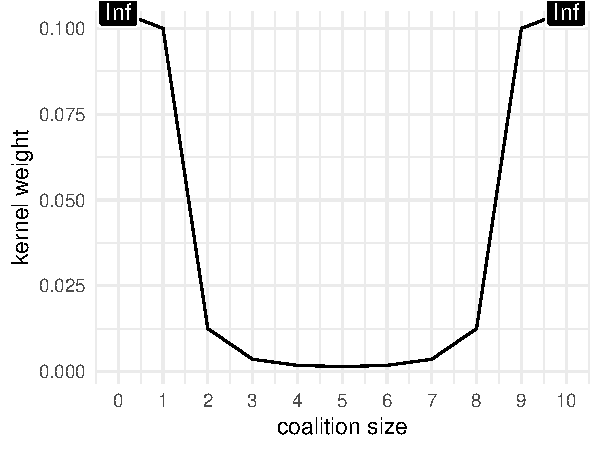
\includegraphics[width=0.6\columnwidth]{figure_man/kernel-weights.pdf}
%     %\caption{Examplary dependence between kernel weights and coalition size for a data set p = 10 features}   
% \end{figure}
% \end{onlyenv}


% \begin{onlyenv}<2>
% \vspace{1cm}
% \begin{exampleblock}{}
% \[
% \tikzmark{pi}\pi_{x}\left(\mathbf{z}^{\prime (k)}\right)=\frac{(
% \tikzmark{M}p-1)}{\left(\begin{array}{c} p \\\left|\mathbf{z}^{\prime (k)}\right|\end{array}\right)\left|
% \tikzmark{z}\mathbf{z}^{\prime (k)}\right|\left(p-\left|\mathbf{z}^{\prime (k)}\right|\right)}
% \]
% \begin{tikzpicture}[
%   remember picture,
%   overlay,
%   expl/.style={draw=blue,fill=white,rounded corners,text width=3cm},
%   arrow/.style={blue,ultra thick,->,>=latex}
% ]
% \node[expl] 
%   (piex) 
%   at (2,2.5cm)
%   {$\pi_x(\mathbf{z}^{\prime (k)})$: kernel weight for coalition $\mathbf{z}^{\prime (k)}$};
% \node[expl] 
%   (Mex) 
%   at (8,3cm)
%   {$p$: Number of features in $\xv$};
% \node[expl] 
%   (zex) 
%   at (6,-1cm)
%   {$\mid \mathbf{z}^{\prime (k)}\mid$: coalition size / sum of 1s in $\mathbf{z}^{\prime (k)}$};
% \draw[arrow]
%   (piex.south) to[out=270,in=135] ([xshift= 0.5ex, yshift=2ex]{pic cs:pi}); 
% \draw[arrow]
%   (Mex.south) to[out=270,in=90] ([xshift= 0.5ex, yshift=2ex]{pic cs:M}); 
% \draw[arrow]
%   (zex.north) to[out=90,in=250] ([xshift= 0.5ex, yshift=-1ex]{pic cs:z}); 
% \end{tikzpicture}
% \end{exampleblock}
% \end{onlyenv}


% % \begin{onlyenv}<3>

% % $$\pi_{x}\left(z^{\prime}\right)=\frac{(M-1)}{\left(\begin{array}{c} M \\\left|z^{\prime}\right|\end{array}\right)\left|z^{\prime}\right|\left(M-\left|z^{\prime}\right|\right)}$$

% % \begin{itemize}
% %     \item If a coalition consists of a single feature, we can learn about this feature’s isolated main effect on the prediction
% %     \item If a coalition consists of all but one feature, we can learn about this feature’s total effect (main effect plus feature interactions)
% %     \item If a coalition consists of half the features, we learn little about an individual feature’s contribution, as there are many possible coalitions with half of the features
% % \end{itemize}
% % \end{onlyenv}

% % \begin{onlyenv}<4>
% % \vspace{1cm}
% % \textbf{Limited Budget $K$}: Can we be a bit smarter about the sampling of coalitions, than just randomly drawing?
% % \begin{itemize}
% %     \item The smallest and largest coalitions take up most of the weight\\ We get better Shapley value estimates by using some of the sampling budget K to include these high-weight coalitions
% %     \item We start with all possible coalitions with 1 and M-1 features, which makes 2 times M coalitions in total\\ When we have enough budget left (current budget is K - 2M), we can include coalitions with 2 features and with M-2 features and so on.
% %     \item From the remaining coalition sizes, we sample with readjusted weights
% % \end{itemize}
% % \end{onlyenv}
  
% \end{frame}


% \begin{frame}{Kernel shap - in 5 steps}
% \textbf{Step 3: Compute weights through Kernel}\\\medskip
% \textbf{Purpose}: to include this knowledge in the local surrogate model (linear regression), we calculate weights for each coalition which are the observations of the linear regression
% \only<1>{    $$\pi_{x}\left(\mathbf{z}^{\prime}\right)=\frac{(p-1)}{\left(\begin{array}{c} p \\|\mathbf{z}^{\prime}|\end{array}\right)|\mathbf{z}^{\prime}|(p-|\mathbf{z}^{\prime}|)} \leadsto \pi_x\left(\mathbf{z}^{\prime} = (1,0,0)\right)=\frac{(3-1)}{\left(\begin{array}{c} 3 \\1\end{array}\right)1\left(3-1\right)} = \frac{1}{3}$$
% }

% \begin{table}[]
%     \centering
%         \begin{tabular}{l |c|ccc|c}
%  Coalition & $\mathbf{z}^{\prime (k)}$ &  hum & temp & ws & weight\\
%   \hline 
%   $\varnothing$ & $\mathbf{z}^{\prime (1)}$ & 0 & 0 & 0 & $\infty$ \\
%   hum & $\mathbf{z}^{\prime (2)}$ & 1 & 0 & 0 & 0.33 \\
%   temp &  $\mathbf{z}^{\prime (3)}$ & 0 & 1 & 0 & 0.33 \\
%   ws &   $\mathbf{z}^{\prime (4)}$ & 0 & 0 & 1 & 0.33  \\
%   hum, temp & $\mathbf{z}^{\prime (5)}$ & 1 & 1 & 0 & 0.33 \\
%   temp, ws & $\mathbf{z}^{\prime (6)}$ & 0 & 1 & 1 & 0.33 \\
%   hum, ws &   $\mathbf{z}^{\prime (7)}$ & 1 & 0 & 1 & 0.33 \\
%   hum, temp, ws & $\mathbf{z}^{\prime (8)}$ & 1 & 1 & 1 & $\infty$ \\
  
 
%   \end{tabular}
% \end{table}
% \medskip
% \only<2>{
% $\leadsto$ weights for empty and full set are infinity and not used as observations for the linear regression\\ $\leadsto$ instead constraints are used such that properties (local accuracy and missingness) are satisfied
% }

  
% \end{frame}

% %\begin{frame}{Coalition Mapping}
% %We define a coalition $z^{\prime}$, by describing a function 

% %$$
% %h\left(z^{\prime}\right)=z \text { where } h:\{0,1\}^{M} \rightarrow \mathbb{R}^{p}
% %$$


% %\begin{onlyenv}<1>
% %\vspace{1cm}
% %\begin{itemize}
% %    \item Coalition $z^{\prime} \in \{0, 1\}^M$ is the  vector, indicating if feature $j$ contributes to the prediction 
% %    \item $h(\cdot)$ represent a function that maps 1’s to the corresponding value from the observation x that we want to explain: $h(\cdot)$ connects our coalition vector to the underlying data 
% %\end{itemize}
% %\end{onlyenv}

% %\begin{onlyenv}<2->
% %\begin{tikzpicture}
% %\centering

% %\node<2> (tab1) {%
% %  \begin{tabular}{l |cccc}
% %  observation & temp & hum & ws & yr\\
% %  \hline 
% %  $x_{ex}$ & 24.7 & 58.5 & 13.96 & 2011\\
%  % \\
%  % \\
%   %\end{tabular}};
% %\node<3-> (tab1) {%
% %  \begin{tabular}{l |cccc}
% %  observation & temp & hum & ws & yr\\
% %  \hline 
% %  $x_{ex}$ & 24.7 & 58.5 & 13.96 & 2011\\
% %  $z_{temp, yr}$ & 24.7 & $\varnothing$ & $\varnothing$ & 2011\\
% %  $z_{yr}$ & $\varnothing$ & $\varnothing$ & $\varnothing$ & 2011\\
% %  \end{tabular}};
% %\node<2> [left=of tab1] (tab2) {%
% %  \begin{tabular}{l |cccc}
% %  Coalition & temp & hum & ws & yr\\
% %  \hline 
% %  $x^{\prime}$ & 1 & 1 & 1 & 1 \\
% %  \\
% %  \\
% %  \end{tabular}};
% %\node<3-> [left=of tab1] (tab2) {%
% %  \begin{tabular}{l |cccc}
% %  Coalition & temp & hum & ws & yr\\
% %  \hline 
% %  $x^{\prime}$ & 1 & 1 & 1 & 1 \\
% %  $z^{\prime}_{temp, yr}$ & 1 & 0 & 0 %& 1 \\
% %  $z^{\prime}_{yr}$ & 0 & 0 & 0 & 1 %\\
% %  \end{tabular}};
% %\draw<2->[->]
% %(tab2.north) to[out=30,in=150] node[below]{$h(\cdot)$} (tab1.north) ;
% %\end{tikzpicture}
% %\end{onlyenv}
% %\begin{onlyenv}<3->
% %\begin{itemize}
% %    \item $h(\cdot)$ maps 1’s to the %corresponding value from the observation x that we want to explain
% %    \item<4> it maps 0’s to the values of another observation that we sample from the data
% %    \item<4>  we equate “feature value is absent” with “feature value is replaced by random feature value from data”
% %\end{itemize}
% %\end{onlyenv}
% %\end{frame}


% \begin{frame}{Kernel shap - in 5 steps}
% \textbf{Step 4: Fit a weighted linear model}\\\medskip
% \textbf{Aim}: Estimate a weighted linear model with Shapley values being the coefficients $\phi_j$
% $$
% g\left(\mathbf{z}^{\prime (k)}\right)=
% \phi_{0}+\sum_{j=1}^{p}
%  \phi_{j} z_{j}^{\prime (k)} \only<2>{\leadsto g\left(\mathbf{z}^{\prime (k)}\right)=
% 4515 +
%  34 \cdot z_{1}^{\prime (k)} - 1654 \cdot z_{2}^{\prime (k)} - 323 \cdot z_{3}^{\prime (k)} }
% $$


% \only<1>{
% and minimize by WLS using the weights $\pi_{x}$ of step 3
%     $$L\left(\hat{f}, g, \pi_{x}\right)=\sum_{k = 1}^K\left[\hat{f}\left(h_{x}\left(\mathbf{z}^{\prime (k)}\right)\right)-g\left(\mathbf{z}^{\prime (k)}\right)\right]^{2} \pi_{x}\left(\mathbf{z}^{\prime (k)}\right)$$

% with $\phi_0 = \E(\fh)$ and $\phi_p = \fh(x) - \sum_{j=0}^{p-1} \phi_j$ we receive a $p-1$ dimensional linear regression problem
% }

% \only<2>{
% \begin{table}[]
%     \centering
%         \begin{tabular}{l |ccc|c|c}
%   $\mathbf{z}^{\prime (k)}$ &  hum & temp & ws & weight & $\fh$\\
%   \hline 
%    $\mathbf{z}^{\prime (2)}$ & 1 & 0 & 0 & 0.33 & 4635\\
%     $\mathbf{z}^{\prime (3)}$ & 0 & 1 & 0 & 0.33 & 3087\\
%      $\mathbf{z}^{\prime (4)}$ & 0 & 0 & 1 & 0.33 & 4359\\
%      $\mathbf{z}^{\prime (5)}$ & 1 & 1 & 0 & 0.33 & 3060\\
%      $\mathbf{z}^{\prime (6)}$ & 0 & 1 & 1 &0.33 & 2623\\
%      $\mathbf{z}^{\prime (7)}$ & 1 & 0 & 1 & 0.33 & 4450\\
%       \multicolumn{1}{c}{} & \multicolumn{3}{c}{\upbracefill}&\multicolumn{1}{c}{} &\multicolumn{1}{c}{\upbracefill}\\[-1ex]
%     \multicolumn{1}{c}{} & \multicolumn{3}{c}{$\scriptstyle input$}&\multicolumn{1}{c}{} &  \multicolumn{1}{c}{$\scriptstyle output$}\\
  
 
%   \end{tabular}
% \end{table}
% }


  
% \end{frame}


% \begin{frame}{Kernel shap - in 5 steps}
% \textbf{Step 5: Return SHAP values}\\\medskip
% \textbf{Intuition}: Estimated Kernel SHAP values are equivalent to Shapley values 
% \begin{align*}
% g(\mathbf{z}^{\prime (8)}) &= \fh(h_x(\mathbf{z}^{\prime (8)}) ) = 4515 + 34 \cdot 1 - 1654 \cdot 1 - 323 \cdot 1\\&= \underbrace{\E(\fh)}_{\phi_0} + \phi_{hum} + \phi_{temp} + \phi_{ws} = \fh(\xv) = 2573
% \end{align*}

% \begin{figure}
%     \centering
%     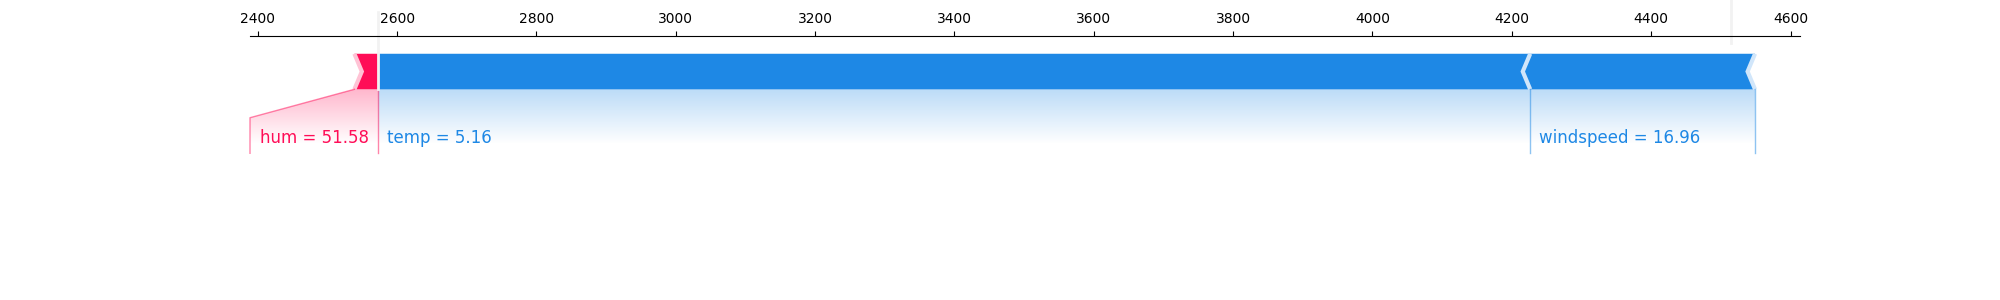
\includegraphics[width=\columnwidth]{figure_man/exSHAP.png}
% \end{figure}

% \end{frame}
% %\begin{frame}{Marginal Contribution}

% %\begin{itemize}
% %    \begin{onlyenv}<1>
% %    \item Consider coalition $z^{\prime}$ as indicator function for our shapley values $\phi$
% %    \end{onlyenv}
% %    \begin{onlyenv}<2>
% %    \item This connects the coalition vector $z^{\prime}$ to the respective marginal contribution
% %    \end{onlyenv}
% %    \begin{onlyenv}<3>
% %    \item To estimate the marginal contribution, we can transfer the coalition to the data space by $h(z^{\prime})$
% %    \end{onlyenv}
% %    \begin{onlyenv}<4->
% %    \item $\fh(h(z^{\prime}))$ connects the coalitions directly to the marginal distribution.
% %    \end{onlyenv}
% %\end{itemize}

% %\vspace{1cm}

% %\begin{tikzpicture}
% %\centering

% %\node<1-2> (tab1) {%
% %  \begin{tabular}{l |cccc}
% %  Coalition & temp & hum & ws & yr\\
% %  \hline 
% %  $x^{\prime}$ & 1 & 1 & 1 & 1 \\
% %  $z^{\prime}_{temp, yr}$ & 1 & 0 & 0 & 1 \\
% %  $z^{\prime}_{yr}$ & 0 & 0 & 0 & 1 \\
% %  \end{tabular}};
% %\node<2-> [right=of tab1] (tab2) {%
% %\begin{tabular}{l | cccc}
% %  & temp & hum & ws & yr\\
% %  \hline 
% %  $g(x^{\prime})$ & $\phi_{temp}$ + & $\phi_{hum}$ + & $\phi_{ws}$ + & $\phi_{yr}$ \\
% %  $g(z^{\prime}_{temp, yr})$ & $\phi_{temp}$ + &  &  & $\phi_{yr}$\\
% %   $g(z^{\prime}_{yr})$ & &  &  & $\phi_{yr}$ \\
% %  \end{tabular}};
% %\node<3-> [left=of tab2] (tab) {%
% %  \begin{tabular}{l |cccc}
% %  observation & temp & hum & ws & yr\\
% %  \hline 
% %  $x_{ex}$ & 24.7 & 58.5 & 13.96 & %2011\\
% %  $z_{temp, yr}$ & 24.7 & %$\varnothing$ & $\varnothing$ & %2011\\
% %  $z_{yr}$ & $\varnothing$ & %$\varnothing$ & $\varnothing$ & 2011\\
% %  \end{tabular}};
% %\draw<2>[->]
% %(tab1.south) to[out=320,in=200] node[above]{$\sum \mathbb{I}_{[z^{\prime}_i == 1]} \phi_i$} (tab2.south) ;
% %\draw<3->[->]
% %(tab2.south) to[out=200,in=330] node[above]{$\fh(h(z^{\prime}))$} (tab1.south) ;
% %\end{tikzpicture}

% %\begin{onlyenv}<4>
% %\begin{equation}
% %\begin{array}{lllc}
  
% %  g(x^{\prime}) &= \phi_{temp} + \phi_{hum} + \phi_{ws} + &\phi_{yr} &= 6825\\
% %  g(z^{\prime}_{temp, yr}) &= \phi_{temp} + &\phi_{yr} &= 6134\\
% %   g(z^{\prime}_{yr}) &= &\phi_{yr} &= 4325\\
% %\end{array}
% %\end{equation}
% %\end{onlyenv}

% %\begin{onlyenv}<5>
% %\vspace{0.5cm}

% %\textbf{Notice:}\\ We created a coalition data set $Z^{\prime}$ here by sampling multiple coalitions from observation $\xv$ that is evaluable with the prediction function $\fh$
% %\end{onlyenv}

% %\end{frame}





\begin{frame}{Properties}

\textbf{Local Accuracy}
$$
f(\xv)=g\left(\xv^{\prime}\right)=\phi_{0}+\sum_{j=1}^{p} \phi_{j} x_{j}^{\prime}
$$
\begin{onlyenv}<1>
\textbf{Intuition:} If the coalition includes all features ($\xv^{\prime}  \in \{1\}^p $), the attributions $\phi_j$ and the null output $\phi_0$ sum up to the original model output $f(\xv)$\\\medskip
Local accuracy corresponds to the \textbf{axiom of efficiency} in Shapley game theory 

\end{onlyenv}

\begin{onlyenv}<2->
\textbf{Missingness}
$$
x_{j}^{\prime}=0 \Longrightarrow \phi_{j}=0
$$
\end{onlyenv}

\begin{onlyenv}<2>
\textbf{Intuition:}  A missing feature gets an attribution of zero
\end{onlyenv}

\begin{onlyenv}<3->
\textbf{Consistency} \\
\end{onlyenv}
\begin{onlyenv}<3>
$\mathbf{z}^{\prime (k)}_{-j} \text{ denotes setting } z_{j}^{\prime (k)}=0$ . For any two
models $\fh$ and $\fh^{\prime}$, if
$$
\fh_{x}^{\prime}\left(\mathbf{z}^{\prime (k)}\right)-\fh_{x}^{\prime}\left(\mathbf{z}^{\prime (k)}_{-j}\right) \geq \fh_{x}\left(\mathbf{z}^{\prime (k)}\right)-\fh_{x}\left(\mathbf{z}^{\prime (k)}_{-j}\right)
$$
for all inputs $\mathbf{z}^{\prime (k)} \in \{0, 1\}^p$, then
$$
\phi_{j}\left(\fh^{\prime}, \mathbf{x}\right) \geq \phi_{j}(\fh, \mathbf{x})
$$
\end{onlyenv}

\begin{onlyenv}<4->
$$
\fh_{x}^{\prime}\left(\mathbf{z}^{\prime (k)}\right)-\fh_{x}^{\prime}\left(\mathbf{z}^{\prime (k)}_{-j}\right) \geq \fh_{x}\left(\mathbf{z}^{\prime (k)}\right)-\fh_{x}\left(\mathbf{z}^{\prime (k)} _{-j}\right) \Longrightarrow \phi_{j}\left(\fh^{\prime}, \xv\right) \geq \phi_{j}(\fh, \xv)
$$

\textbf{Intution:} If a model changes so that the marginal contribution of a feature value increases or stays the same, the Shapley value also increases or stays the same\\\medskip 
From \textbf{consistency} the Shapley \textbf{axioms of additivity, dummy and symmetry} follow
\end{onlyenv}


\end{frame}

%\begin{frame}{Tree SHAP \citebutton{Lundberg et al 2018}{https://doi.org/10.48550/arXiv.1802.03888}}

%TreeSHAP is a fast model specific exact calculation of Shapley values for tree based models 

%\begin{onlyenv}<1-3>
%\vspace{0.5cm}
% Consider following Tree:

% \textbf{Cases}
% Consider the following cases of feature subset S

% \begin{itemize}
%     \begin{onlyenv}<1>
%     \item  S is the set of all features – 
%     the prediction from the node in which the observation x falls is be the expected prediction.
%     \end{onlyenv}
%     \begin{onlyenv}<2>
%     \item S is empty -
%     use the weighted average of predictions of all terminal nodes in the decision tree. \\
     
%     \end{onlyenv}
%     \begin{onlyenv}<3>
%     \item S contains some, but not all, features -
%     ignore predictions of unreachable nodes \& average the predictions item from the remaining terminal nodes weighted by  sizes
%     \end{onlyenv}
% \end{itemize}

% Given observation $x_{ey}$ and the displayed tree
% \begin{table}
% \begin{columns}[T]
% \begin{column}{0.3\textwidth}
% \centering
% \begin{tabular}{l |rrr}
%   \hline
%   & temp & year & $\fh$\\ 
%   \hline
%  $x_{ex}$ & 24.27 & 2011 & 6825 \\ 
%  \hline
% \end{tabular}
% \end{column}
% \begin{column}{0.7\textwidth}
% \begin{tikzpicture}[
%     node/.style={%
%       draw=blue,
%       rectangle,
%       fill=white,
%       rounded corners
%     },
%   ]
% \centering
%     \node [node, label=below:{\scriptsize n=10}] (A) {year $>$ 2011};
%     \path (A) ++(7:3.8cm) node [node, label=below:{\scriptsize n=5}] (B) {count = 3200};
%     \path (A) ++(-7:3.8cm) node [node, label=below:{\scriptsize n=5}] (C) {temp $>$ 30};
%     \path (C) ++(14:3.8cm) node [node, label=below:{\scriptsize n=3}] (D) {count = 6850};
%     \path (C) ++(0:3.8cm) node [node, label=below:{\scriptsize n=2}] (E) {count = 5400};
    

%     \draw (A) -- node [above] {\scriptsize no}(B);
%     \draw (A) -- node [above, yshift=-0.1cm] {\scriptsize yes}(C) ;
%     \draw (C) -- node [above] {\scriptsize no} (D);
%     \draw (C) -- node [above, yshift=-0.1cm] {\scriptsize yes}(E);
    
% \end{tikzpicture}
% \end{column}
% \end{columns}
% \end{table}

% \begin{onlyenv}<1>
% $$
% S = \varnothing \rightarrow z^{\prime} = (0, 0) \rightarrow \phi_0 = \frac{3200*5 + 6850*3 +5400*2}{10}= 3775
% $$
% \end{onlyenv}

% \begin{onlyenv}<2>
% $$
% S = \{x_{temp}, x_{year}\} \rightarrow z^{\prime} = (1, 1)  \rightarrow \phi_{year, temp} = 6850
% $$
% \end{onlyenv}

% \begin{onlyenv}<3>
% $$
% S = \{x_{temp}\} \rightarrow z^{\prime} = (0, 1)  \rightarrow \phi_{\cdot, temp} = \frac{3200*5 + 3* 6850}{8} = 3625
% $$
% \end{onlyenv}
% \end{onlyenv}

% \begin{onlyenv}<4>
% \vspace{1.5cm}
% \textbf{Complexity:}
% \begin{itemize}
%     \item Complexity of exact KernelSHAP: $\mathcal{O}(TLD^2)$
%     \item Complexity of TreeSHAP: $\mathcal{O}(TL2M)$
% \end{itemize}

% T is the number of trees, L is the maximum number of leaves in any tree and D the maximal depth of any tree
% \end{onlyenv}


% \end{frame}

\endlecture
\end{document}
